\chapter{Implementacja systemu}

Rozdział ten opisuje implementację zrealizowanego w ramach pracy systemu. Jego działanie obejmuje następujące kroki: 
\begin{enumerate}
\item Na początku użytkownik wybiera choroby, na które choruje pacjent. 
\item Następnie program wyświetla graficzną reprezentację wytycznych dla wskazanych chorób oraz wyświetla listy pól wyboru, które pozwalają na udzielanie odpowiedzi na pytania zawarte w wytycznych. 
\item Po udzieleniu odpowiedzi na wybrane pytania (informacja nie musi być kompletna) program rozwiązuje problem CLP, w wyniku którego uzyskujemy listę konfliktów, które wystąpiły między wytycznymi oraz grafy wynikowe z wprowadzonymi zmianami. 
\item Po uzyskaniu rozwiązania problemu można wybrać inne odpowiedzi na pytania i wygenerować nowe rozwiązania problemu. Można także wybrać inne choroby i powiązane z nimi wytyczne.
\end{enumerate}
Poszczególne kroki zostały szczegółowo opisane w punkcie \ref{sec:kroki}. 

Program przetwarza wytyczne reprezentowane w postaci grafu skierowanego, w którym mogą wystąpić następujące rodzaje węzłów:
\begin{itemize}
\item \textit{węzeł początkowy} i \textit{końcowy} oznaczający odpowiednio rozpoczęcie i zakończenie wytycznych,
\item \textit{węzeł kontekstowy} opisujący chorobę, dla której sformułowane są wytyczne,
\item \textit{węzeł akcji} definiujący akcję (podanie leku, badanie, procedura), jaką należy wykonać,
\item \textit{węzeł decyzyjny} wskazujący na dane opisujące pacjenta, które należy pozyskać i sprawdzić w celu wyboru jednego z kilku możliwych sposobów postępowania,
\item \textit{węzeł równoległy} rozpoczynający lub kończący ścieżki równoległe.
\end{itemize}

Wszystkie węzły mają unikalne identyfikatory. Ponadto łuki (w dalszej części tekstu będziemy stosowali określenie krawędzie) wychodzące z węzłów decyzyjnych opisane są za pomocą etykiet odpowiadających poszczególnym decyzjom. Wreszcie węzły akcji i decyzyjne posiadają dodatkowe etykiety z dodatkowym, czytelnym ich opisem. Przykładowy graf przedstawiono na rys. \ref{fig:sciezki_rownolegle}. 

Grafy przechowywane są w plikach w formacie DOT. Format ten nie pozwala na użycie dodatkowej informacji semantycznej o typach węzłów (można określić jedynie ich identyfikatory oraz etykiety). Aby odróżnić węzły równoległe od decyzyjnych, sprawdzane są ich etykiety (a dokładnie ich dostępność lub brak). Poza tym, aby odróżnić węzeł rozpoczynający ścieżki równoległe od węzła kończącego, sprawdzane są liczby krawędzi wchodzących i wychodzących. Węzeł rozpoczynający ścieżki równoległe charakteryzuje się tym, że nie ma etykiety oraz posiada więcej niż jedną krawędź wyjściową. Natomiast węzeł kończący ścieżki równoległe nie posiada etykiety, ma więcej niż jedną krawędź wejściową oraz liczba jego krawędzi wyjściowych jest większa od zera (liściem jest zawsze węzeł końcowy).

\begin{figure}[H]
\centering
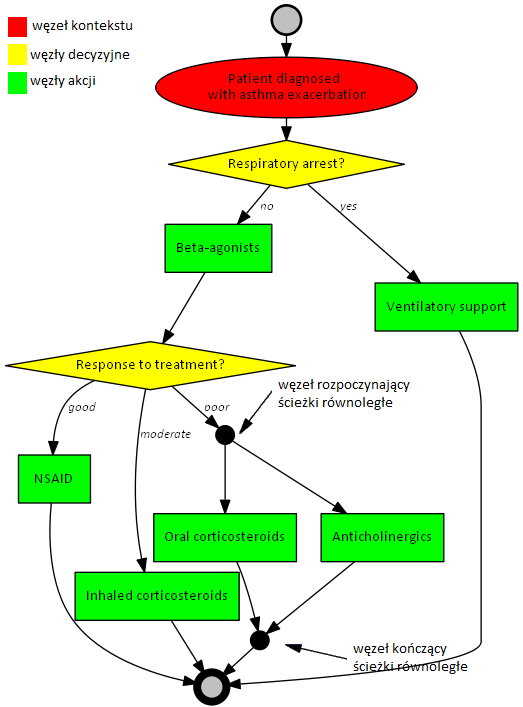
\includegraphics[width=0.7\textwidth]{img/asthma_sciezki_rownolegle.png}
\caption{Przykład ścieżek równoległych}
\label{fig:sciezki_rownolegle}
\end{figure}

W dalszych opisach wykorzystano pojęcia \textit{terapia} oraz \textit{element terapii}. \textit{Terapia} jest to pojedyncza ścieżka w grafie. \textit{Element terapii} natomiast to dla węzłów decyzji identyfikator węzła i etykieta wybranej krawędzi oddzielone znakiem zapytania, dla pozostałych węzłów \textit{elementem terapii} jest identyfikator węzła.

\section{Wykorzystywane dane}


Dane wykorzystywane oraz generowane przez program znajdują się w następujących katalogach:
\begin{itemize}
\item{\texttt{Algorytmy} – katalog zawiera pliki o rozszerzeniu DOT opisujące grafy reprezentujące dostępne wytyczne kliniczne,}
\item{\texttt{Konflikty} – katalog zawiera opisy konfliktów, jakie mogą wystąpić między wytycznymi oraz definicje zmiany, które należy wprowadzić w przypadku wystąpienia tych konfliktów,}
\item{\texttt{Grafy} – katalog zawiera zmodyfikowane grafy chorób przedstawiające aktualnie przebytą ścieżkę oraz grafy wynikowe prezentujące rozwiązania. Grafy są w dwóch formatach – tekstowym w formacie DOT oraz graficznym w formacie PNG. Podczas kończenia pracy programu zawartość tego katalogu jest kasowana}
\end{itemize}

\section{Główne klasy}
Program zaimplementowano w języku Java. Poniżej przedstawiono listę głównych klas wykorzystywanych w programie (i pojawiających się w dalszych opisach):
\begin{itemize}
\item{\texttt{AddToTherapy} - dodawanie identyfikatorów węzłów do listy opisującej konkretną terapię,}
\item{\texttt{ChocoClass} - rozwiązanie problemu CLP za pomocą solvera Choco,}
\item{\texttt{Color} - kolorowanie wierzchołków i krawędzi grafów,}
\item{\texttt{CreateTherapies} - generowanie terapii,}
\item{\texttt{ExecuteInteractions} - wprowadzanie zmian w terapiach w przypadku wykrycia konfliktów, }
\item{\texttt{GoForward} - przechodzenie do kolejnego węzła decyzyjnego, }
\item{\texttt{GraphFunctions} - przydatne metody związane z grafami, np. znalezienie węzłów docelowych określonego węzła,}
\item{\texttt{ImageGraph} - wyświetlanie grafów, }
\item{\texttt{MainClass} - obsługa przejścia między poszczególnymi krokami działania programu,}
\item{\texttt{RadioButtonList} - tworzenie i obsługa zdarzeń list pól wyboru służących do udzielania odpowiedzi na pytania,}
\item{\texttt{Results} - wyświetlanie wyników,}
\item{\texttt{Window} - główne okno programu.}
\end{itemize}

\section{Główne kroki działania}
\label{sec:kroki}

\subsection{Wybór chorób}
Celem tego kroku jest wybór tych wytycznych, które będą brane pod uwagę przy ustalaniu terapii. W katalogu \texttt{Algorytmy} program szuka plików posiadających rozszerzenie DOT. Dla każdego takiego pliku tworzone jest pole wyboru. Pole wyboru posiada etykietę równą nazwie choroby. Utworzone pole wyboru jest następnie dodawane do globalnej listy 
pól wyboru \texttt{Window.checkBoxGroup} oraz do panelu 
znajdującego się w lewym górnym rogu okna programu (rys. \ref{fig:wybor_chorob}). 
\begin{figure}[H]
\centering
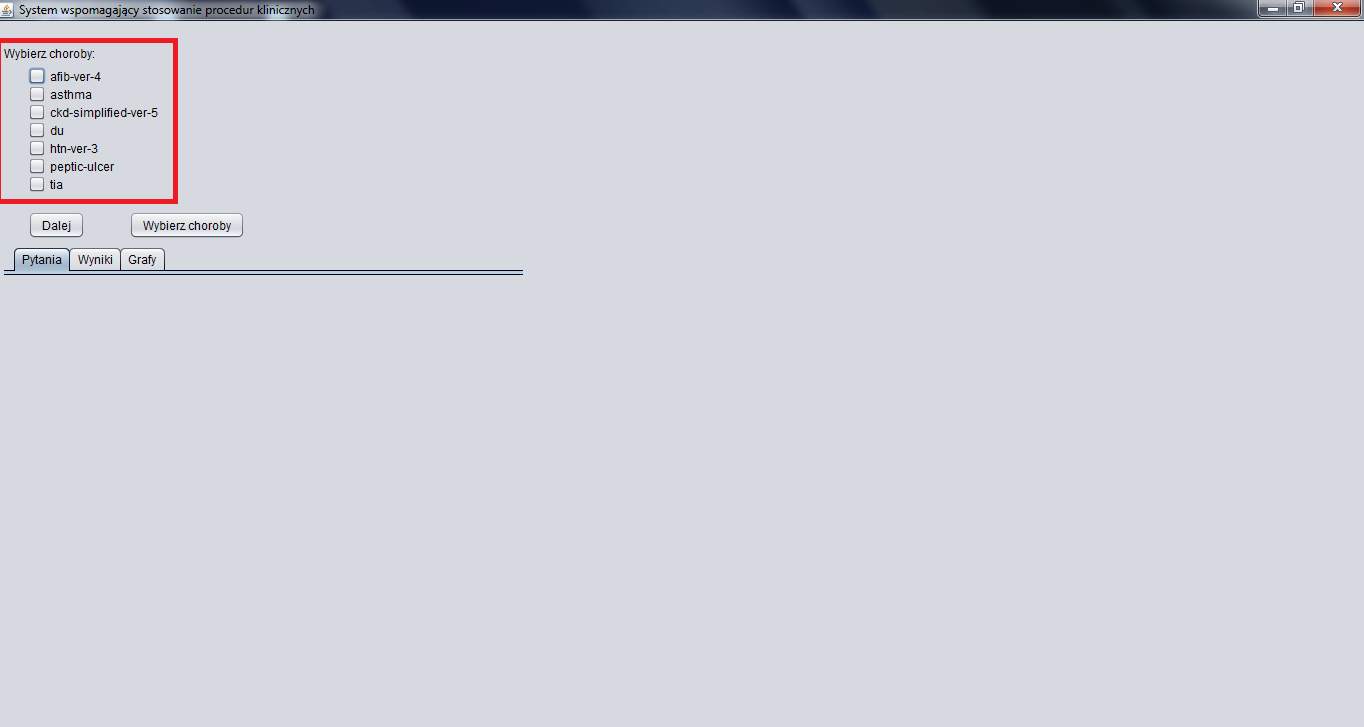
\includegraphics[width=\textwidth]{img/wybor_chorob.png}
\caption{Panel wyboru chorób}
\label{fig:wybor_chorob}
\end{figure}
Po wybraniu chorób, tzn. po kliknięciu w odpowiednie pola wyboru i kliknięciu przycisku „Dalej”, nazwy wybranych chorób są dodawane do listy \texttt{MainClass.selectedDiseases} i program przechodzi do fazy wyświetlania grafów oraz udzielania odpowiedzi na pytania. 

\subsection{Wyświetlanie grafów oraz udzielanie odpowiedzi na pytania}
Ten krok pozwala na utworzenie graficznej reprezentacji wytycznych oraz wybór ścieżki w grafie (terapii) zgodnej z dostępnymi danymi pacjenta. Po wybraniu chorób i kliknięciu przycisku „Dalej” program dla każdej choroby odczytuje za pomocą metody \texttt{GraphFunctions.getGraph} grafy z plików w formacie DOT. Następnie program pobiera korzenie każdego z grafów za pomocą metody \texttt{GraphFunctions.get\-StartNode}, a potem wywołuje metodę \texttt{GoForward.goForward}, która przemieszcza się po grafie (startując w jego korzeniu) do momentu, gdy napotka pierwszy węzeł decyzji. 

Metoda \texttt{goForward} dodaje aktualny węzeł do listy elementów terapii. Następnie wykonuje pętlę \texttt{while}, której warunek kontynuacji obejmuje trzy przypadki. Pierwszy warunek sprawdza, czy węzeł posiada jedną krawędź wyjściową. Drugi warunek sprawdza, czy węzeł rozpoczyna ścieżki równoległe, a trzeci czy węzeł kończy ścieżki równoległe. 

Wewnątrz pętli wykonywane są następujące akcje. Po pierwsze wykonywana jest kolejna, wewnętrzna pętla \texttt{while} (jej warunek jest taki sam, jak pierwszy z warunków w pętli zewnętrznej), aby dodać do listy elementów terapii wszystkie węzły, które mają tylko jedną krawędź wyjściową, czyli droga w grafie, po której należy się poruszać jest jednoznacznie określona. Po wykonaniu tej pętli \texttt{goForward} zatrzymuje się na węźle, który jest liściem (nie posiada żadnej krawędzi wyjściowej), albo ma więcej niż jedną krawędź wyjściową.

Następnie następuje sprawdzenie, czy aktualny węzeł rozpoczyna ścieżki równoległe (jest to też drugi warunek w pętli zewnętrznej). Jeśli warunek ten jest spełniony, wywoływana jest metoda \texttt{parallel\-Path}. Metoda ta jest wywoływana również w dla trzeciego przypadku, czyli gdy uzyskany węzeł kończy ścieżki równoległe, a program nie przeszedł jeszcze przez wszystkie ścieżki równoległe. Metoda \texttt{GoForwared.parallel\-Path} jest w postaci pętli \texttt{while}, która działa dopóki program nie przejdzie przez wszystkie ścieżki równoległe związane z aktualnym węzłem i uzyskany węzeł nie jest węzłem decyzyjnym. Wszystkie przebyte po drodze węzły dodawane są do listy elementów terapii.  

Po wywołaniu metody \texttt{goForward} program wywołuje metodę \texttt{Color.color}, która zaznacza przebytą ścieżkę w grafie kolorując oraz pogrubiając kontury przebytych węzłów oraz przebyte krawędzie.
 
Po wywołaniu metody \texttt{color} wywołana zostaje metoda \texttt{ImageGraph.newImageGraph}, której zadaniem jest wygenerowanie i wyświetlenie nowego obrazu grafu. Na początku metoda zapisuje do pliku wynik metody \texttt{toString} wywołanej dla grafu. Następnie wywoływana jest metoda \texttt{ImageGraph.getImageGraphPath}, która uruchamia zewnętrzny program \texttt{dot} i tworzy z zapisanego wcześniej pliku tekstowego graf w postaci obrazu w formacie PNG. W kolejnym kroku metoda \texttt{ImageGraph.newImageGraph} tworzy obiekt klasy \texttt{BufferedImage} z wygenerowanym w poprzednim kroku obrazem. Później metoda dokonuje skalowania obrazu tak, aby mógł on się zmieścić w oknie (a dokładnie w przeznaczonym dla niego polu). 

Jeśli szerokość lub wysokość obrazu przekracza ustalony próg, obraz zmniejszany jest do 2/3 wielkości tak, aby był on czytelny (w tym przypadku do pola z obrazem dodawane są suwaki). Ponadto, jeżeli szerokość i wysokość obrazu jest mniejsza od wielkości pola, to na etykiecie umieszczany jest obraz bez skalowania (tzn. w skali 1:1).
 
Ostatnim krokiem jest wywołanie metody \texttt{RadioButtonList.createRadioButtonList}. Metoda ta dla każdego elementu terapii, który posiada znak zapytania tworzy panel. Elementy terapii zwierające znak zapytania odpowiadają krokom decyzyjnym. Pierwszym elementem panelu jest etykieta węzła. Pozostałe elementy stanowią pola wyboru z etykietami, których wartości są równe etykietom krawędzi wychodzących z węzła decyzyjnego. Do tych pól wyboru dodawany jest jeszcze jedno z etykietą „brak wartości”, przydatne w sytuacji, gdy dane nie są znane. Na końcu tworzony jest jeszcze jeden panel, tym razem dla pytania, na które jeszcze nie została udzielona odpowiedź -- dla niego zaznaczone jest pole wyboru z etykietą „brak wartości”. Przy pierwszym wyświetleniu grafu tworzony jest tylko ten panel. Ponadto, do każdego pola wyboru podczepiana jest metoda \texttt{RadioButtonList.updateRadioButtonList} obsługująca zdarzenia związane ze zmianą wartości pola.

Po wywołaniu metoda \texttt{updateRadioButtonList} na początku szuka elementu w liście elementów terapii, którego dotyczy wybrane pytanie (i związane z nim pole wyboru). Jeśli zaznaczone pole wyboru ma etykietę „brak wartości”, usuwane są wszystkie elementy terapii od elementu, którego dotyczy wybrane pytanie, do ostatniego elementu listy pytań. Innymi słowy następuje cofnięcie się w grafie, co oznacza, że pytania i odpowiedzi znajdujące się „poniżej” wybranej lokalizacji są odrzucane.

Jeśli natomiast zaznaczone pole wyboru nie posiada etykiety równej „brak wartości” i nie istnieje element na liście elementów terapii, który jest związany z pytaniem (użytkownik odpowiada na to pytanie po raz pierwszy), to do tej listy dodawany jest element o wartości równej \texttt{question?answer}, gdzie \texttt{answer} jest etykietą krawędzi, z którą związane jest zaznaczone pole wyboru.  Jeśli natomiast istnieje element związany z pytaniem (użytkownik modyfikuje wcześniej udzieloną odpowiedź), to w liście elementów terapii podmieniany jest element, który jest związany z pytaniem na wartość \texttt{question?answer}, a następnie usuwane są wszystkie elementy listy terapii, które się znajdują za podmienionym elementem (analogicznie jak w przypadku wyboru „braku wartości”). 

Następnie aktualnym węzłem staje się węzeł, do którego dochodzi krawędź związana z wybraną odpowiedzią (tzn. krawędź o etykiecie \texttt{answer} wychodzącej z węzła o identyfikatorze \texttt{question}). Węzeł ten jest punktem startowym dla kolejnego wywołania metody \texttt{goForward}. Metoda \texttt{goForward} nie jest wywoływana, gdy pole wyboru ma etykietę „brak wartości”. Potem metoda \texttt{updateRadio\-ButtonList} koloruje graf na nowo na podstawie zaktualizowanej listy elementów terapii. Tworzony jest także nowy obraz grafu za pomocą metody \texttt{newImageGraph}. Na końcu tworzona jest nowa lista pytań i odpowiedzi za pomocą metody \texttt{createRadioButtonList}. 

Zaktualizowane grafy prezentowane są po prawej stronie ekranu na osobnych zakładkach. Każda zakładka dotyczy wytycznych związanych z jedną z wybranych chorób. Z lewej strony ekranu pojawiają się natomiast zakładki z listami pytań i pól wyboru pozwalającymi na uzupełnienie danych pacjenta. W tym przypadku również jedna zakładka dotyczy jednej choroby. Przykładowy ekran z grafami i polami wyboru przedstawiono na rys. \ref{fig:wyswietlanie_grafow}.
\begin{figure}[H]
\centering
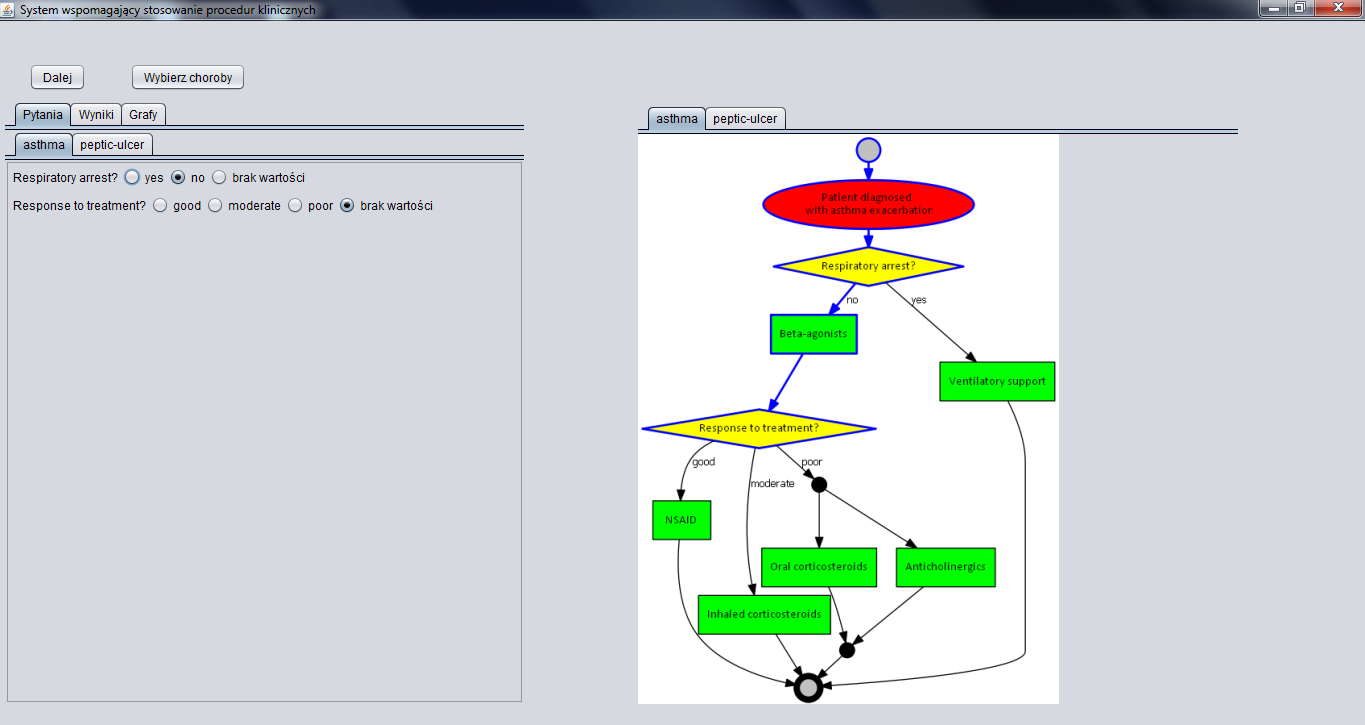
\includegraphics[width=\textwidth]{img/wyswietlanie_grafow.png}
\caption{Wyświetlanie grafów}
\label{fig:wyswietlanie_grafow}
\end{figure}

\subsection{Wyszukiwanie konfliktów}
Celem tego kroku jest znalezienie konfliktów pojawiających się między wytycznymi. Wyszukiwanie konfliktów rozpoczyna się od metody ChocoClass.solve. Na początku program szuka w katalogu \texttt{Konflikty} plików opisujących konflikty i sposoby ich rozwiązania, które można zastosować do aktualnego zestawu wytycznych. Nazwa każdego pliku opisującego konflikty składa się z listy nazw chorób oddzielonych przecinkami (konflikty pojawiają się między wytycznymi dla tych chorób). Jeśli jakakolwiek choroba z tej listy została wybrana podczas działania programu chorobach, plik zostaje użyty. 

Plik z konfliktami zawiera jeden lub więcej wpisów (każdy poświęcony jednemu konfliktowi), a wpis (umieszczony w jednej linii) składa się z dwóch części. Pierwsza część zawiera elementy, których jednoczesne wystąpienie powoduje konflikt. Elementy te są oddzielone spacjami. Druga część zawiera zmiany, jakie należy wprowadzić w przypadku zaistnienia konfliktu. Zmiany te są oddzielone od siebie przecinkami. Jeśli plik zostaje użyty, do listy \texttt{conflictsList} dodawane są konflikty, a do listy \texttt{interactionsList} zmiany. Ponadto, do listy \texttt{additionalQuestions} dodawane są te elementy opisujące konflikt, które oznaczają dodatkowe pytania (tzn. odwołują się do danych, które jawnie nie występują w wytycznych) -- nazwy tych elementów rozpoczynają się znakiem „\&”. Wreszcie zanegowane elementy konfliktów (rozpoczynające się od „not”) dodawane są do listy \texttt{notConflictElems}. Następnie program tworzy okienko dialogowe, które pozwala udzielić odpowiedzi na dodatkowe pytania. Pytania mogą być dwóch typów. Pierwszy typ występuje, gdy odpowiedni element konfliktu nie posiada znaku równości, mniejszości ani większości. Wtedy udzielana odpowiedź ma postać tak/nie. Drugi typ to „zmienna operator liczba”. Operator może być postaci „=”, „>”, „<”, „>=” lub „<=”. Dla tego typu elementu podawana jest wartość liczbowa w okienku dialogowym, a program sprawdza czy podana liczba spełnia warunek występujący w elemencie. 

Po udzieleniu odpowiedzi na wszystkie dodatkowe pytania program przechodzi do kolejnej części wyszukiwania konfliktów zrealizowanej w metodzie \texttt{ChocoClass.solveNextPart}. Metoda ta najpierw wywołuje metodę \texttt{ChocoClass.findSolutions}, która dla każdego możliwego konfliktu (odczytanego z pliku) wykonuje szereg operacji. Najpierw sprawdza, czy konflikt znajduje się na liście \texttt{foundConflicts}. Lista \texttt{foundConflicts} zawiera rzeczywiste konflikty, które zostały dotychczas zidentyfikowane przez program (tutaj należy zaznaczyć, że nie każdy możliwy konflikt musi zachodzić). Jeśli konflikt nie znajduje się na tej liście tworzony jest obiekt klasy \texttt{Solver}. Następnie dodawane są zmienne na podstawie wcześniej udzielonych odpowiedzi na dodatkowe pytania. Dokonuje tego metoda \texttt{ChocoClass.setAdditionalVariables}. Metoda ta sprawdza, czy pytanie jest typu tak/nie lub czy odpowiedzią na pytanie jest wartość liczbowa. W pierwszej sytuacji, jeśli odpowiedź jest równa tak, program tworzy zmienną typu \texttt{IntVar} o wartości równej jeden. Jeżeli odpowiedź jest równa nie, program tworzy zmienną \texttt{IntVar} o wartości równej zero. Jeśli odpowiedzią na pytanie jest wartość liczbowa, program tworzy zmienną \texttt{IntVar} o wartości równej podanej liczbie. 

Po wykonaniu metody \texttt{setAdditionalVariables} program wywołuje metodę \texttt{setVariables}. Metoda ta dla każdych wytycznych tworzy tablicę terapii. Dla każdej terapii (w ramach poszczególnych wytycznych) tworzona jest zmienna \texttt{IntVar} o nazwie \textit{<choroba>\_terapia<n>}, gdzie \textit{choroba} jest nazwą choroby, a \textit{n} jest indeksem terapii. Zmienna ta przyjmuje wartości zero, gdy  określona terapia nie zostaje użyta lub jeden, gdy zostaje użyta. Zmienna jest zapisywana w tablicy terapii. Następnie metoda tworzy listę \texttt{notConflictElemsTherapy}, do której dodawane są te elementy konfliktu z listy \texttt{notConflictElems}, które nie znajdują się na liście elementów konkretnej terapii, ale znajdują się w grafie związanym z terapią (innymi słowy są to te elementy, które występują w pozostałych terapiach dla danych wytycznych). 

Metoda \texttt{setVariables} tworzy też tablicę \texttt{vars}, która będzie zawierała zmienne wchodzące w skład pojedynczej terapii. Dla każdego elementu listy \texttt{notConflictElemsTherapy} w tablicy \texttt{vars} zapisywane są zmienne o nazwie \textit{not\_<X>}, gdzie X jest elementem terapii z \texttt{notConflictElems\-Therapy}. Zmienna ta przyjmuje wartość 0, gdy zmienna związana z elementem terapii jest równa 1 i odwrotnie. Ponadto, dla każdego elementu terapii zapisywana jest zmienna w tablicy \texttt{vars}. Jeśli zmienna odnosi się do elementu terapii (akcji) oznaczającego podanie leku, w ramach której określono jego dawkę, tworzona jest zmienna \textit{<X>\_dosage}, gdzie \textit{X} jest elementem terapii. Następnie metoda dodaje ograniczenie mówiące, że zmienna \textit{<choroba>\_terapia<n>} przyjmuje wartość jeden, tylko wtedy, gdy suma zmiennych należących do tablicy \texttt{vars} jest równa wielkości tej tablicy (innymi słowy, gdy udało się przejść przez całą ścieżkę odpowiadającą terapii i jednocześnie nie wystąpił żaden z zanegowanych elementów konfliktu). W przeciwnym razie \textit{<choroba>\_terapia<n>} przyjmuje wartość zero. Po przejściu przez wszystkie terapie dla danych wytycznych metoda dodaje ograniczenie polegające na tym, że suma zmiennych terapii choroby ma być równa jeden, czyli dla każdej choroby ma zostać użyta tylko jedna terapia. 

Po wykonaniu metody \texttt{setVariables} program dodaje ograniczenia odpowiadające konfliktom. Najpierw dodawane są ograniczenia dla tych możliwych konfliktów, których udało się uniknąć (tzn. po uwzględnieniu związanych z nimi ograniczeń udało się uzyskać poprawne rozwiązanie -- konflikty takie znajdują się na liście \texttt{avoidedConflicts}). Następnie w metodzie \texttt{ChocoClass.set\-ConflictConstraint} dodawane jest ograniczenie dla konfliktu sprawdzanego w aktualnej iteracji pętli. Najpierw tworzy ona listę \texttt{constraintsList} przechowującą to ograniczenie. Następnie metoda iteracyjnie przetwarza elementy wchodzące w skład aktualnego konfliktu:
\begin{itemize}
\item Jeśli element konfliktu jest zanegowany (jego opis zaczyna się od „not”), do listy \texttt{constraints\-List} dodawane jest ograniczenie \textit{not(<X> = 1)}, gdzie \textit{X} jest elementem terapii wymienionym w elemencie konfliktu. 
\item Jeśli element konfliktu zawiera jeden z operatorów „<”, „<=”, „=”, „>”, lub „>=” wówczas wywoływana jest metoda \texttt{ChocoClass.conflictWithDosage}, która sprawdza, jaki charakter ma element terapii z elementu konfliktu i dodaje odpowiednie ograniczenia do \texttt{constraints\-List}. Jeśli element terapii jest związany z dodatkowym pytaniem (jego nazwa rozpoczyna się od „\&”), wówczas dodawane jest ograniczenie \textit{<X> <operator> <wartość>}, gdzie \textit{X} jest elementem terapii, a \textit{wartość} jest liczbą występującą w elemencie konfliktu. W przeciwnym razie (element terapii jest związany z akcją, w tym z podaniem leku), do \texttt{constraintsList} dodawane są dwa ograniczenia. Pierwsze jest w postaci \textit{<X> = 1} (odpowiada ono wykonaniu wskazanej akcji), natomiast drugie ma formę \textit{<X>\_dosage <operator> <wartość>} i dotyczy dawki związanej z daną akcją. 
\item W pozostałych przypadkach do \texttt{constraintsList} dodawane jest ograniczenie \textit{<X> = 1}, gdzie \textit{X} to odpowiedni element terapii.
\end{itemize}

Po zakończeniu przetwarzania poszczególnych elementów konfliktu do obiektu klasy \texttt{Solver} dodawane jest ograniczenie w formie \textit{not(and(\texttt{constraintsList}))}, aby zabezpieczyć się przed wystąpieniem aktualnego konfliktu.

Następnie wywoływana jest metoda \texttt{findSolution}, która szuka rozwiązania problemu. Jeśli rozwiązanie istnieje, aktualny konflikt dodawany jest to listy do \texttt{avoided\-Conflicts}. Jeśli natomiast rozwiązanie nie istnieje, aktualny konflikt jest dodawany do \texttt{foundConflicts}, a do listy \texttt{interactionsList} dopisywane są zmiany powiązane z danym konfliktem. Ponadto, gdy nie ma rozwiązania program wywołuje metodę \texttt{ExecuteInteractions.execute\-Interactions}, która dokonuje zmian w wytycznych (a dokładnie w terapiach), a także program wywołuje rekurencyjnie metodę \texttt{findSolutions}, aby sprawdzić, czy wprowadzone zmiany nie spowodowały wystąpienia konfliktów, które zostały wcześniej sprawdzone, oraz aby sprawdzić kolejne konflikty. 

Ostatecznie, program znajduje rozwiązania problemu z ograniczeniami dla tych konfliktów, które znajdują się na liście \texttt{avoidedConflicts} (jak już wspomniano, są to konflikty, których udało się uniknąć -- dla konfliktów, które wystąpiły, wprowadzono odpowiednie zmiany do terapii). Po wygenerowaniu pierwszego rozwiązania program tworzy listę o nazwie \texttt{solutions}. Następnie w pętli, która działa dopóki istnieje kolejne rozwiązanie, program zapisuje do zmiennej \texttt{solution} nazwy zmiennych, które w rozwiązaniu posiadają wartość równą jeden. Następnie, jeśli zmienna \texttt{solution} nie znajduje się jeszcze w liście \texttt{solutions}, dodawana jest do tej listy. 

Na końcu program do listy \texttt{therapies} dodaje rozwiązania. Polega to na tym, że dla każdego rozwiązania z listy \texttt{solutions} znajdujemy odpowiadające mu terapie w liście \texttt{therapiesDiseases}. Lista \texttt{therapiesDiseases} zawiera terapie wszystkich wybranych chorób zgodne z udzielonymi odpowiedziami na pytania znajdujące się w wytycznych. Znalezienie odpowiedniej terapii polega na odczycie nazwy choroby i identyfikatora terapii ze zmiennych <choroba>\_terapia<n> znajdujących się w liście \texttt{solutions}.

\subsection{Wyświetlanie wyników}
\label{sect:revisions}
Ostatni krok polega na wyświetleniu grafów wynikowych prezentujących rozwiązania, a także utworzeniu listy znalezionych konfliktów wraz z wprowadzanymi zmianami. Program prezentuje wyniki za pomocą metody \texttt{Results.setResults}. Na początku metoda wywołuje inną metodę o nazwie \texttt{Results.setGraphs}. Zajmuje się ona modyfikowaniem grafów, wprowadzając niezbędne zmiany usuwające znalezione konflikty.
Dla każdej modyfikacji sprawdzany jest jej typ, który może być jednym z następujących:
\begin{itemize}
\item \textit{replace <X> with <Y>}, gdzie węzeł \textit{X} zamienia się na węzeł \textit{Y},
\item \textit{add <X> before/after <Y>}, gdzie węzeł \textit{X} jest dodawany przed lub po elemencie \textit{Y},
\item \textit{remove <X>}, węzeł \textit{X} jest usuwany,
\item \textit{increase\_dosage/decrease\_dosage <X> <DV>}, gdzie dawka leku z węzła \textit{X} jest zwiększana lub zmniejszana o wartość \textit{DV},
\item \textit{change\_dosage <X> <V>}, gdzie dawka leku z węzła \textit{X} jest ustalana na \textit{V}.  
\end{itemize}

Zmiana grafu uzależniona jest od typu modyfikacji i przeprowadzana jest w następujący sposób:
\begin{itemize}
\item Dla modyfikacji \textit{replace}, najpierw wyszukiwany jest węzeł \textit{X}. Po znalezieniu takiego węzła z pliku \texttt{Konflikty/nazwy.txt} odczytywana jest etykieta węzła \textit{Y}. Wreszcie identyfikator i etykieta znalezionego węzła są zmieniane na nowe wartości. 
\item Dla modyfikacji \textit{add}, poszukiwany jest węzeł \textit{Y}, przed lub za którym ma zostać umieszczony nowy węzeł \textit{X}. Następnie program tworzy węzeł \textit{X}, nadaje mu etykietę pobraną z pliku \texttt{nazwy.txt} i dodaje węzeł do grafu. Jeśli węzeł \textit{X} jest wstawiany po elemencie postaci \textit{pytanie?odpowiedź}, wówczas staje się on węzłem docelowym dla krawędzi z etykietą \textit{odpowiedź}, oraz wstawiana jest dodatkowa krawędź od węzła \textit{X} do poprzedniego węzła docelowego. W przeciwnym razie wstawiana jest krawędź z Y do X (dla \textit{add after}) lub z X do Y (dla \textit{add before}).
\item Dla modyfikacji \textit{remove} atrybuty usuwanego węzła \textit{X} modyfikowane są w taki sposób, że węzeł staje się niewidoczny na wynikowym grafie
\item Dla modyfikacji \textit{increase\_dosage}, \textit{decrease\_dosage} i \textit{change\_dosage} odpowiednio zmienia się końcową część etykiety zmienianego węzła \textit{X}, gdzie w nawiasach kwadratowych umieszczona jest zmieniona dawka leku związanego z węzłem. 

\end{itemize}

Na zakończenie metoda \texttt{setGraphs} dla każdego grafu wywołuje metodę \texttt{color} zaznaczającą przebyte węzły i krawędzie, a następnie metodę \texttt{newImageGraph}, która powoduje wygenerowanie grafu w postaci obrazkowej. 

Po wywołaniu metody \texttt{setGraphs} program tworzy także tekstową reprezentację uzyskanych rozwiązań. Dla każdej z otrzymanych terapii obejmuje ona identyfikatory oraz etykiety elementów terapii (czyli odwiedzonych węzłów w grafach). Reprezentacja ta zawiera również opis napotkanych konfliktów oraz listę wprowadzonych zmian. Przy ustalaniu etykiet węzłów grafach wykorzystywane są informacje z pliku \texttt{nazwy.txt}.


\section{Przykład działania programu}
W tym punkcie przedstawiono działanie programu na wybranym przykładzie klinicznym obejmującym wytyczne dla dwóch chorób: migotania przedsionków (ang. \textit{atrial fibrillation}, rys. \ref{fig:afib_przyklad}) oraz przewlekłej choroby nerek (ang. \textit{chronic kidney disease}, rys. \ref{fig:ckd_przyklad}). W przypadku węzłów odpowiadających akcjom i decyzjom podano ich etykiety oraz identyfikatory (w nawiasach okrągłych).

\begin{figure}[H]
\centering
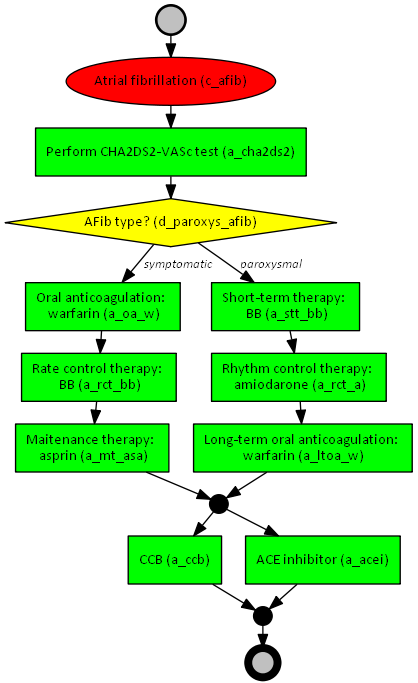
\includegraphics[scale=0.5]{img/afib-ver-4_przyklad.png}
\caption{Wytyczne dla migotania przedsionków}
\label{fig:afib_przyklad}
\end{figure}
\begin{figure}[H]
\centering
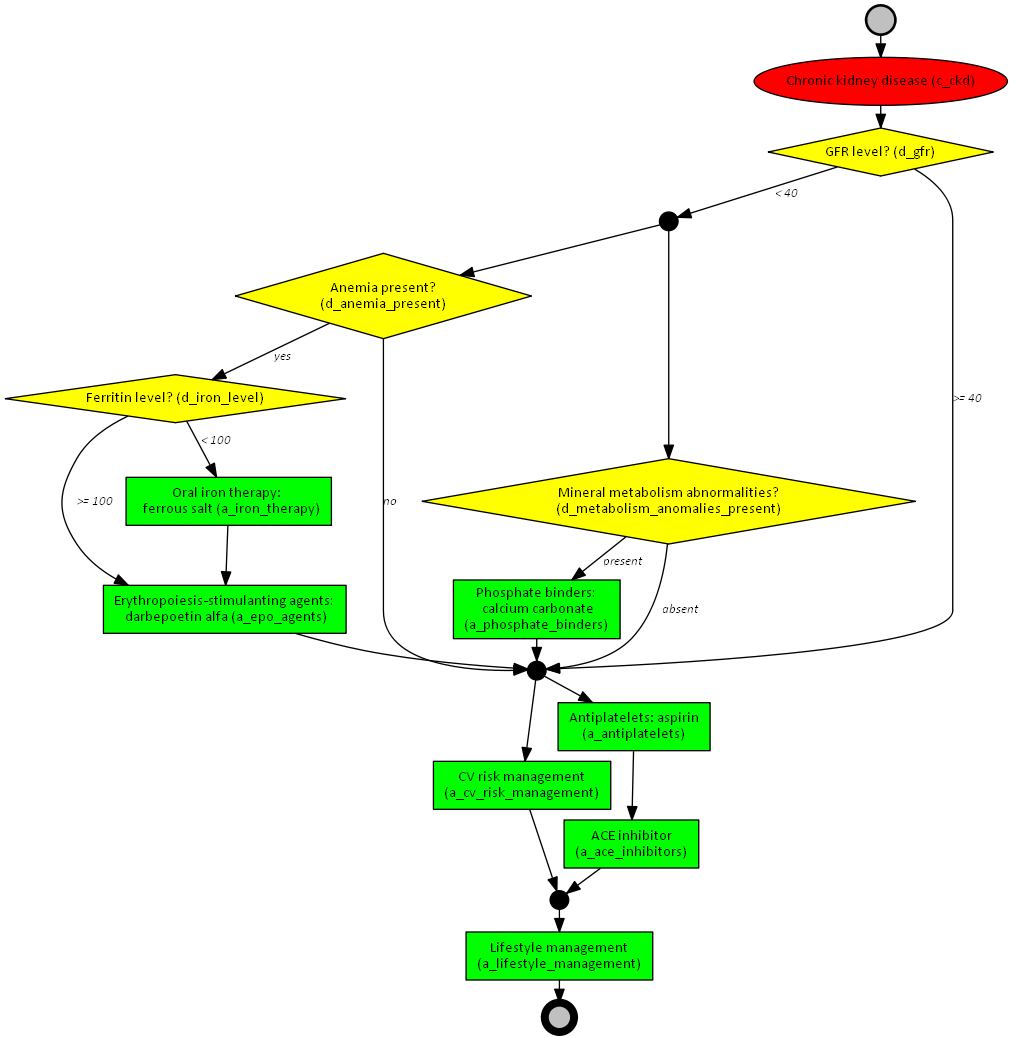
\includegraphics[scale=0.4]{img/ckd-simplified-ver-5_przyklad.png}
\caption{Wytyczne dla przewlekłej choroby nerek}
\label{fig:ckd_przyklad}
\end{figure}

W przypadku wytycznych dla migotania przedsionków (rys. \ref{fig:afib_przyklad}) program zatrzymuje się na pierwszym węźle decyzyjnym \textit{AFib type?}, zapisując wcześniej do listy elementów terapii węzeł startowy, węzeł kontekstowy określający chorobę oraz węzeł \textit{Perform CHA2DS2-VASc test}. Po wskazaniu przez użytkownika odpowiedzi \textit{paroxysmal} program dodaje do listy \textit{d\_afib?paroxysmal}, a następnie trzy węzły: \textit{Short-term therapy: BB}, \textit{Rhythm control therapy: amiodarone} i \textit{Long-term oral anticoagulation: warfarin}. Następnie program dodaje węzeł rozpoczynający ścieżki równoległe, następnie dwa węzły znajdujące się na ścieżkach równoległych (najpierw węzeł \textit{CCB}, następnie węzeł \textit{ACE inhibitor}), a później węzeł kończący ścieżki równoległe. Ostatecznie program dodaje węzeł końcowy grafu. 

W wytycznych dla choroby nerek (rys. \ref{fig:ckd_przyklad}) program zatrzymuje się na węźle decyzyjnym \textit{GFR level?}, dodając po drodze do listy elementów terapii węzeł startowy oraz węzeł choroby. Po udzieleniu odpowiedzi \textit{<40} program dodaje do listy \textit{d\_gfr?<40}, a następnie trafia na węzeł rozpoczynający ścieżki równoległe, który również jest dodawany do listy. W kolejnym kroku program zatrzymuje się na  decyzji znajdującej się na lewej ścieżce równoległej: \textit{Anemia present?}. Po uzyskaniu odpowiedzi \textit{no} program dodaje do listy element \textit{d\_anemia\_present?no}, a następnie wraca do prawej ścieżki równoległej i zatrzymuje się na decyzji \textit{Mineral metabolism abnormalities?}. Po uzyskaniu odpowiedzi \textit{absent} program dodaje do listy \textit{d\_metabolism\_anomalies\_present?absent}. Następnie program umieszcza na liście węzeł kończący ścieżki równoległe, który jednocześnie rozpoczyna kolejne ścieżki równoległe. W kolejnym kroku program dodaje element znajdujący się na lewej ścieżce równoległej, czyli \textit{CV risk management}, a następnie elementy znajdujące się na prawej ścieżce równoległej, czyli \textit{Antiplatelets: aspirin} oraz \textit{ACE inhibitor}. Ostatecznie dodawany jest węzeł kończący ścieżki równoległe, węzeł \textit{Lifestyle management} oraz węzeł końcowy grafu.

Po określeniu terapii program przechodzi do fazy wyszukiwania konfliktów. Najpierw program odczytuje plik z konfliktami dotyczącymi migotania przedsionków, przewlekłej choroby nerek oraz nadciśnienia. Plik ten ma następującą zawartość:
\begin{verbatim}
c_htn c_ckd:remove a_step1_acei,remove a_step1_ccb
c_afib c_ckd c_htn:remove a_step3_diuretric
c_afib c_ckd:replace a_antiplatelets with a_warfarin,replace a_rct_a with a_bb
c_afib c_ckd &CHA2DS2-VASc>2:replace a_mt_asa with a_warfarin_2
c_afib c_ckd &CHA2DS2-VASc<=1:replace a_oa_w with a_aspirin_1,
replace a_ltoa_w with a_aspirin_2
\end{verbatim}
Następnie program prosi o uzupełnienie danych pacjenta poprzez podanie wartości zmiennej \textit{CHA2\-DS2-VASc}. Użytkownik uzupełnia dane -- niech wartość tej zmiennej będzie równa 5, a program zaczyna wyszukiwać konflikty. Ostatecznie program znajduje dwa konflikty: (\textit{c\_afib c\_ckd} -- współwystąpienie obu chorób) oraz (\textit{c\_afib c\_ckd \&CHA2DS2-VASc>2} -- podwyższona wartość CHA2DS2-VASc w połączeniu z migotaniem przedsionków). Pierwsze dwa konflikty nie wystąpiły, ponieważ pacjent nie choruje na nadciśnienie (\textit{c\_htn}), więc odpowiednie wytyczne nie są rozważane. Ostatni konflikt nie wystąpił natomiast dlatego, że zmienna CHA2DS2-VASc przyjmuje wartość większą od 1.

W kolejnym kroku program tworzy zmodyfikowane grafy wynikowe, które zawierają zmiany wprowadzone w celu uniknięcia konfliktów. Graf dla migotania przedsionków został przedstawiony na rys. \ref{fig:afib_rozw}, natomiast graf dla przewlekłej choroby nerek jest na rys. \ref{fig:ckd_rozw}. W grafie dla migotania przedsionków węzeł \textit{Maintenance therapy: aspirin} został zmieniony na \textit{Maintenance therapy: Warfarin} oraz węzeł \textit{Rhytm control therapy: amiodarone} na węzeł \textit{BB}. Natomiast W grafie dla przewlekłej choroby nerek węzeł \textit{Antiplatelets: aspirin} został zmieniony na \textit{Warfarin}.

\begin{figure}[H]
\centering
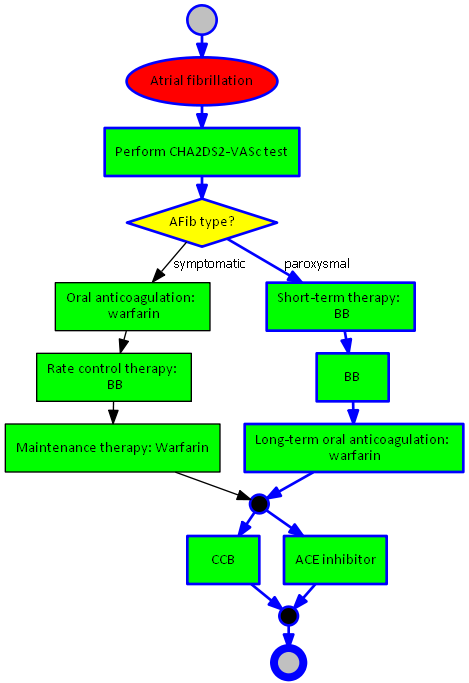
\includegraphics[scale=0.5]{img/rozwiazanie1afib-ver-4_przyklad.png}
\caption{Wytyczne dla migotania przedsionków}
\label{fig:afib_rozw}
\end{figure}
\begin{figure}[H]
\centering
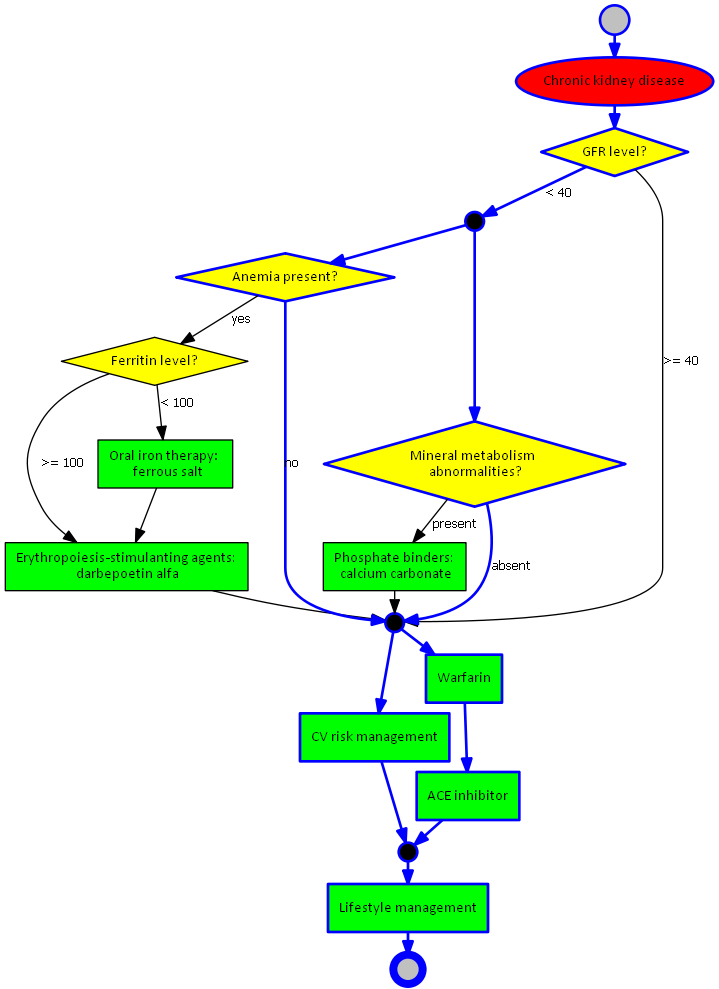
\includegraphics[scale=0.4]{img/rozwiazanie1ckd-simplified-ver-5_przyklad.png}
\caption{Wytyczne dla przewlekłej choroby nerek}
\label{fig:ckd_rozw}
\end{figure}